\documentclass[tikz,border=8pt]{standalone}
\usetikzlibrary{arrows.meta,positioning,calc}
\begin{document}
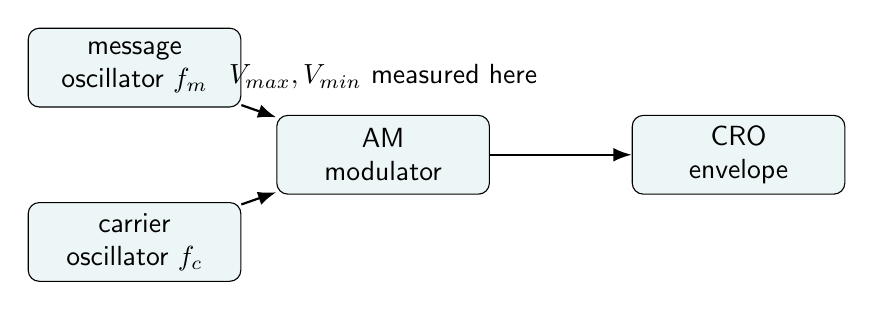
\begin{tikzpicture}[font=\sffamily,>=Latex,box/.style={draw,rounded corners,minimum height=10mm,minimum width=27mm,align=center,fill=teal!7}]
\node[box] (msg) {message\\oscillator $f_m$};
\node[box] (car) [below=12mm of msg] {carrier\\oscillator $f_c$};
\node[box,right=18mm of $(msg)!0.5!(car)$] (mod) {AM\\modulator};
\node[box,right=18mm of mod] (cro) {CRO\\envelope};
\draw[thick,-Latex] (msg)--(mod);
\draw[thick,-Latex] (car)--(mod);
\draw[thick,-Latex] (mod)--(cro);
\node[above=2mm of mod,align=center] {$V_{max},V_{min}$ measured here};
\end{tikzpicture}
\end{document}
